\documentclass[czech]{article}
\usepackage{listings}
%\documentstyle[epsf,epic,eepic,eepicemu]{article} \oddsidemargin=-5mm
\usepackage{graphicx}
\usepackage[utf8]{inputenc} % LaTeX source encoded as UTF-8
\oddsidemargin=-5mm
\evensidemargin=-5mm\marginparwidth=.08in \marginparsep=.01in
\marginparpush=5pt\topmargin=-15mm\headheight=12pt
%\headsep=25pt\footheight=12pt \footskip=30pt\textheight=25cm
\textwidth=17cm\columnsep=2mm
\columnseprule=1pt\parindent=15pt\parskip=2pt

\newcommand{\graphsperthread}{50}
\newcommand{\graphspermpiproc}{80}

\begin{document}
\begin{center}
\bf Semestrální projekt MI-PDP 2016/2017:\\[5mm]
    Paralelní algoritmus pro řešení problému maximálního bipartitiního podgrafu\\[5mm] 
       Martin Melka\\[2mm]
magisterské studium, FIT ČVUT, Thákurova 9, 160 00 Praha 6\\[2mm]
\today
\end{center}

\section{Definice problému a popis sekvenčního algoritmu}

\subsection{Definice problému}
Řešení problému maximálního bipartitního podgrafu (MBG) znamená nalézt takový podgraf H daného grafu G, který je bipartitní a jeho počet hran je maximální, tj. neexistuje žádný další bipartitní podgraf grafu G, který by měl větší počet hran než H. Množinu hran grafu H označme F.

Graf je bipartitní právě tehdy, když lze všechny jeho uzly obarvit dvěma barvami.

Jelikož je vstupní graf souvislý, lze určit spodní mez počtu hran řešení. Tou bude $|F|=n-1$, kde $n$ je počet hran grafu. Toto řešení je dáno tím, že pro každý souvislý graf lze najít kostru, tedy takový podgraf, který je strom. Kostru pak stačí "zakořenit", uzly uspořádat do úrovní, jak je u stromů zvykem, a každou úroveň obarvit jinou barvou než tu předchozí.

\subsection{Formát vstupních dat}
Formát vstupních dat je daný zadáním:
\begin{itemize}
	\item Na prvním řádku je číslo $n$, určující počet hran grafu G
	\item Na následujících $n$ řádcích je vždy $n$ číslic $0$ nebo $1$, které reprezentují matici sousednosti grafu -- $1$ znamená, že odpovídající uzly mezi sebou mají hranu, $0$ že nemají.
\end{itemize}

\subsection{Formát výstupních dat}
Formát výstupních dat má následující strukturu:

\begin{verbatim}
Best bipartite graph edge count:
================
==   25 edges ==
================
Bipartite subsets:
0) 0  4  6  7  9  14  1  11  3
1) 2  8  10  12  13  15  5

Edges in bipartite subgraph:
0 <-> 2
0 <-> 8
(...)


Computation time:
13.0867
\end{verbatim}

\noindent Kde: 
\begin{itemize}
	\item Ohraničená hodnota udává počet hran nalezeného grafu,
	\item množiny čísel pod \texttt{Bipartite subsets} ukazují, do které ze dvou množin ten který uzel patří (tj. kterými barvami jsou uzly obarveny),
	\item seznam dvojic čísel udává, mezi kterými uzly jsou ve výsledném grafu hrany,
	\item a nakonec je uveden čas v sekundách, jež byl potřeba pro dokončení výpočtu.
\end{itemize}
\subsection{Popis sekvenčního algoritmu}
Algoritmus řešící problém MBG sekvenčně využívá prohledávání do hloubky, případně do šířky. Detailní popis těchto metod není předmětem tohoto předmětu, jelikož už byly popsány dříve (BI-PA2, BI-ZUM, BI-EFA, BI-GRA).

K reprezentaci uzlů prohledávaného stavového prostoru jsem zvolil matici sousednosti. Z hlediska implementace to znamená to, že každý stav je reprezentován třídou \texttt{Graph}, jež si uchovává vlastní kopii dvourozměrného pole -- matici sousednosti. Kromě toho má některé pomocné metody, například pro ověření, zda je tento graf bipartitní, spojitý, či nespojitý (metoda vrací hodnoty $1$, $0$, resp. $-1$ jako příznak těchto vlastností).

\subsubsection{Generování stavů}
V každém kroku DFS je nutné vygenerovat potomky řešeného stavu (grafu), které se vloží do zásobníku a budou dále zpracovávat. Algoritmus, kterým jsem se rozhodl tyto sousedy-potomky generovat zajišťuje, že množina vygenerovaných podgrafů bude disjunktní -- tedy že žádné dva grafy nebudou totožné, což by v případě jednoduchého odebírání hran nastávalo.

Algoritmus generování funguje tak, že ze zadaného grafu postupně odebírá hrany, čímž generuje podgrafy. Hrany jsou odebírány následujícím způsobem -- každý graf má indexy \texttt{startI} a \texttt{startJ} do matice sousednosti. Ty určují, od které pozice v matici dále budou odebírány hrany (tj. měněny jedičky na nuly). Na předchozí hrany algoritmus nesmí sahat.

Vygenerování množiny potomků stavu s grafem \texttt{G} pak znamená:
\begin{lstlisting}[tabsize=2,language=python]
	given graph G:
	
	neighbors = []
	foreach (i,j)>(startI,startJ):
		if edge(i,j) is present:
			new_graph = G.remove_edge(i,j)
			new_graph.startI = i
			new_graph.startJ = j
			neighbors.append(new_graph)
			
\end{lstlisting}
Tímto způsobem generuji stavy, které může mít dále smysl prohledávat.


\subsubsection{Ořezávání stavového prostoru}
Před samotným zpracováním vygenerovaných stavů je vhodné provést kontrolu, zda to má vůbec smysl:
\begin{itemize}
	\item Pokud je graf bipartitní, nemá smysl prohledávat jeho potomky -- budou mít určitě menší počet hran a tento graf bude tedy zaručeně lepší.
	\item Pokud má graf stejný nebo menší počet hran než dosud nejlepší nalezený graf, nemá smysl ho dále prohledávat.
	\item Pokud je vygenerovaný graf nespojitý, nemá smysl se s ním dále zabývat - zajímají mě pouze spojité grafy. Test spojitosti provádím v rámci testu bipartity, viz popis reprezentace uzlu výše.
	\item Pokud má graf méně hran než $|V|-1$, nemá smysl se s ním zabývat, jelikož toto je spodní mez řešení.
\end{itemize}

\subsection{Naměřené časy}
Časy naměřené na vzorových datech na lokálním stroji (frekvence CPU 2.4GHz) jsou následující:

\begin{itemize}
	\item \texttt{graph10\_5.txt} -- 1020 ms
	\item \texttt{graph17\_3.txt} -- 10 ms
	\item \texttt{graph20\_3.txt} -- 120 ms
	\item \texttt{graph25\_3.txt} -- 130 ms
	\item \texttt{graph14\_4.txt} -- 1650 ms
\end{itemize}

\section{Popis paralelního algoritmu a jeho implementace v OpenMP}

Paralelní algoritmus v OpenMP, tj. řešení se sdílenou pamětí, jsem řešil dvěma způsoby -- pomocí task paralelismu a datového paralelismu.

\textit{Task paralelismus} jsem řešil jednoduše vytvářením nového \texttt{OMP Task} při každém rekurzivním volání DFS funkce. Až na toto tvoření tasků a uzamykání aktualizace nejlepšího řešení do kritické sekce, bylo toto řešení totožné se sekvenčním.

\textit{Datový paralelismus} byl implementačně o něco náročnější než \textit{Task paralelismus}. Pro jeho korektní běh bylo nejprve nutné vygenerovat dostatečně velkou množinu počátečních (disjunktních) stavů, nad kterou poté budou OpenMP vlákna iterovat. Generování počátečních stavů jsem extrahoval do samostatné funkce, která ale vnitřně funguje velmi podobně běžnému BFS algoritmu. Prohledávání probíhá stejně jako u "ostrého" řešení s tím, že ve chvíli, kdy velikost fronty grafů čekajících na zpracování odpovídá zadanému parametru, algoritmus na její konec vloží nedozpracovaný graf (abych nepřišel o žádný ze stavů) a celou frontu vrátí jako výsledek funkce. Nad touto frontou grafů pak standardně pomocí \texttt{\#pragma omp parallel for} spustím požadovaný počet vláken.

Tím, že vlákna mají disjunktní množinu počátečních stavů, které jsou na sobě nezávislé, nemusí na sebe nijak čekat (vyjma kritické sekce při nalezení nového maxima).

Počet generovaných stavů jsem empiricky stanovil na \graphsperthread{}násobek počtu vláken, ale ideální hodnota tohoto parametru silně závisela na vstupních datech.

\subsection{Příkazová řádka}
Kompilace a spuštění programu v příkazové řádce se provede následující sekvencí příkazů:
\begin{verbatim}
	$ cd project
	$ make clean && make
	$ ./solver <input-graph> [seq|omp|mpi] [num_threads]
\end{verbatim}

\noindent Druhý parametr programu udává:
\begin{itemize}
	\item \textbf{seq} -- sekvenční běh.
	\item \textbf{omp} -- běh pouze v OpenMP (nepoužívají se volání MPI).
	\item \textbf{mpi} -- běh OpenMP + MPI (viz dále).
\end{itemize}

V případě použití parametrů \texttt{omp} nebo \texttt{mpi} je ještě nutné udat parametr \texttt{num\_threads}, který určuje, kolik vláken se má na každém výpočetním uzlu spustit.

\section{Popis paralelního algoritmu a jeho implementace v MPI}
Paralelní algoritmus v MPI umožňuje počítat distribuovaně na více výpočetních uzlech. Jedná se o algoritmus s distribuovanou pamětí -- každý z uzlů má svou vlastní a je třeba řešit jejich synchronizaci.

Výpočet maxima na každém z uzlů probíhá totožně jako v předchozím případě algoritmu OpenMP. Rozdíl je v tom kdy a s jakými parametry se tyto OpenMP výpočty spouštějí. To je řízeno komunikací uzlů v MPI. V této části popíšu způsob, jakým tato komunikace probíhá.

Obecný popis algoritmu je takový, že Master proces na začátku výpočtu vygeneruje počáteční stavy. Slave procesy si je od Mastera postupně odebírají a sami je u sebe řeší v OpenMP. Mastera notifikují o nově nalezených maximech a zároveň jsou od něj informováni o nových maximech, nalezených jinými Slavy. Master sám počítá, pokud nejsou žádné Slave procesy, které by potřebovaly novou práci.

\subsection{Master proces}
Master proces je proces s MPI rankem 0. Na začátku výpočtu standardním způsobem uvedeným výše vygeneruje počáteční grafy. Empiricky jsem jejich počet stanovil jako \graphspermpiproc{}násobek počtu MPI procesů. V tuto chvíli Slave procesy nic nedělají. Po vygenerování stavů Master přejde do své výpočetní smyčky, která je zjednodušeně pseudokódem zapsána takto:

\begin{lstlisting}[tabsize=2,language=python]
while not done:
	if message_pending:
		if message_is(slave_needs_work):
			if initial_graphs.size() > 0:
				send_work(slave_id, initial_graphs.pop())
			else:
				send_no_more_work(slave_id)
				if all_slaves_received_no_more_work:
					done = true
					
		elif message_is(slave_finished_computing):
			candidate_graph = receive_result(slave_id)
			if candidate_graph > current_best:
				current_best = candidate_graph
				
	else:  # No pending messages -> start computing on Master node
		if initial_graphs.size() > 0:
			work_graph = initial_graphs.pop()
			computeOpenMP(work_graph, current_best)
\end{lstlisting}

Smyčka se ukončí, pokud byly všechny grafy zpracovány a všem Slave procesům odeslána zpráva \texttt{no\_more\_work}. Po jejím skončení je nalezeno nejlepší řešení, protože byl prohledán celý (ořezaný) stavový prostor.

\subsection{Slave proces}
Slave proces je komplementární k Masteru. Jeho výpočetní smyčka vypadá takto:
\begin{lstlisting}[tabsize=2,language=python]
while not done:
	work = request_work()
	if work is NO_MORE_WORK:
		break  # No more work to be done, quit loop
		
	my_best = computeOpenMP(work.graph, work.master_best)
	send_result(my_best)
\end{lstlisting}

Zde je smyčka jednodušší, Slave jen dokola žádá o práci a počítá. Spolu s prací Master vždy pošle i doposud nejlepší řešení, které si Slave uloží a použije pro ořezání stavového prostoru.

\subsection{Formát MPI zpráv}
Pro komunikaci v MPI používám hlavně jeden typ zprávy - Graf. Ta obsahuje zakódovaný objekt grafu a metadata. Kromě tohoto typu zprávy pak jen zprávy obsahující příznak (\texttt{tag}) -- to jsou zprávy žádosti o práci a oznámení o tom, že žádná práce již není k dispozici.

Formát zprávy s grafem má tento formát:
\begin{itemize}
	\item \texttt{int[5]}: \begin{enumerate}
		\item Počet hran nejlepšího zatím nalezeného řešení (používá se jen při zasílání grafu od Master pro Slave proces)
		\item Počet uzlů posílaného grafu
		\item \texttt{startI}
		\item \texttt{startJ}
		\item Počet hran posílaného grafu (šlo by spočítat z poslané matice, ale tímto se šetří výpočetní čas)
	\end{enumerate}

	\item \texttt{bool[n]}, kde \texttt{n} je počet uzlů grafu -- první řádek matice sousednosti 
	\item \texttt{bool[n]} -- druhý řádek matice sousednosti
	\item \texttt{...}
\end{itemize}

\subsection{Příkazová řádka}
Příkazy pro program jsou popsané v sekci výše. Pokud chci program spustit ve více procesech (pro MPI komunikaci), lze použít tuto konstrukci:
\begin{lstlisting}[tabsize=2]
	$ mpirun -n <process_count> ./solver input/graph mpi <threads_per_process>
\end{lstlisting}

\section{Naměřené výsledky a hodnocení}
\subsection{Vstupní data}
Běh algoritmu jsem měřil na třech vstupních grafech, těmi byly:
\begin{itemize}
	\item \texttt{graph14\_5} - vzorový vstup, graf o 14 uzlech.
	\item \texttt{custom\_14\_5\_10} - vygenerovaný graf s parametry -n 14 -k 5, graf o 14 uzlech.
	\item \texttt{custom\_16\_5} - vygenerovaný graf s parametry -n 16 -k 5, graf o 16 uzlech.
\end{itemize}

Rozdělení výpočetních jader je uvedeno v tabulce \ref{cores-distribution}. Naměřené časy v těchto konfiguracích jsou detailně rozepsány v tabulce \ref{times-table} a zobrazeny v grafu \ref{times-graph}. 

\subsection{Parametry škálování}
Parametry pro škálování výpočtu jsou následující:
\begin{itemize}
	\item \textbf{Počet vygenerovaných grafů na jedno vlákno} (v rámci výpočtu OpenMP) -- \graphsperthread
	\item \textbf{Počet vygenerovaných grafů pro každý MPI proces} -- \graphspermpiproc
\end{itemize}



\subsection{Výsledky}
\begin{table}[]
	\centering
	\caption{Rozdělení výpočetních jader}
	\label{cores-distribution}
	\begin{tabular}{|l||l|l|}
		\hline
		Počet jader & Počet vláken & Počet MPI procesů \\ \hline \hline
		1           & 1            & 1                 \\ \hline 
		2           & 2            & 1                 \\ \hline
		4           & 4            & 1                 \\ \hline
		8           & 4            & 2                 \\ \hline
		16          & 4            & 4                 \\ \hline
		24          & 4            & 6                 \\ \hline
		32          & 8            & 4                 \\ \hline
		60          & 10           & 6                 \\ \hline
	\end{tabular}
\end{table}

\begin{table}[]
	\centering
	\caption{Čas výpočtu algoritmu}
	\label{times-table}
	\begin{tabular}{|r||l|l|l|}
		\hline
		& \multicolumn{3}{c|}{Čas výpočtu {[}s{]}} \\ \hline \hline
		Počet jader & Graf 1    & Graf 2   & Graf 3            \\ \hline
		1           & 423,91    & 386,853  & 1309,21           \\
		2           & 403,442   & 720,561  & 491,596           \\
		4           & 389,849   & 732,664  & 604,743           \\
		8           & 767,365   & 418,172  & \textgreater1800  \\
		16          &           &          &                   \\
		24          &           &          &                   \\
		32          &           &          &                   \\
		60          &           &          &                   \\ \hline
	\end{tabular}
\end{table}

Z naměřených dat je vidět, že paralelizace s výše uvedenými parametry (počty grafů na vlákno a proces) je neefektivní. Nejen, že je sublineární, v některých případech je dokonce pomalejší, než sekvenční řešení. Nejjednodušším způsobem optimalizace pro 1-4 výpočetní jádra by bylo spuštění programu jen s OpenMP. Algoritmus, který byl použit pro naměření těchto výsledků, vždy běžel v MPI módu -- v případě jediného MPI uzlu tedy celý výpočet probíhal jen v Master MPI procesu a v algoritmu se zbytečně volaly MPI metody \texttt{MPI\_Iprobe}.

Při 8 jádrech jsou již použity dva MPI uzly, každý se 4 vlákny. V grafech 1 a 3 došlo k poměrně znatelnému zhoršení výpočetní doby, v grafu 2 se doba zlepšila, ale stále byla delší než sekvenční řešení.

\subsection{Možnosti zlepšení}
Jak již jsem zmínil výše, velkou roli v době výpočtu hrály parametry pro počet generovaných počátečních grafů v závislosti na počtu vláken a procesů. Hodnoty použité pro výpočet jsem experimentálně stanovil na základě výpočtů na svém počítači, kde byl MPI paralelismus simulován pouze na jednom CPU se dvěma vlákny. 

Pro zlepšení získaných časů by tedy bylo vhodné experimentovat s nastaveními těchto parametrů, ale tyto experimenty není v dobu odevzdávání zprávy možné uskutečnit, protože fronta čekajících výpočtů na clusteru STAR je neúnosně velká. Nezbyl mi tak dostatek času na optimalizaci časů pro dané vstupní grafy.

Samotný algoritmus komunikace mezi MPI procesy rovněž poskytuje prostor pro zlepšení. Poté, co Slave proces dokončí výpočet zadaného grafu, odešle o tom Master procesu informaci. Master by mohl ihned zaslat další práci Slave procesu, ale místo toho čeká, až o ni Slave sám požádá.

Další možností pro experimentování by byla úprava Master procesu tak, aby vůbec nepočítal. Mám podezření, že zejména při vyšším počtu MPI uzlů Slave procesy zbytečně čekají na dokončení výpočtu.

\begin{figure} 
	\centering
	\caption{Graf rychlosti výpočtu}
	\label{times-graph}
	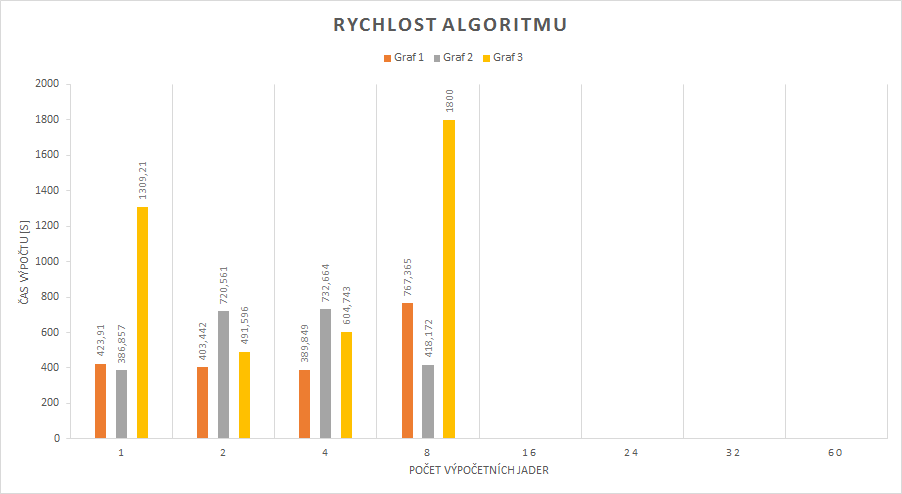
\includegraphics[width=\textwidth]{graph/times-chart.png}
\end{figure}

\begin{figure} 
	\centering
	\caption{Graf zrychlení výpočtu}
	\label{speedup-graph}
	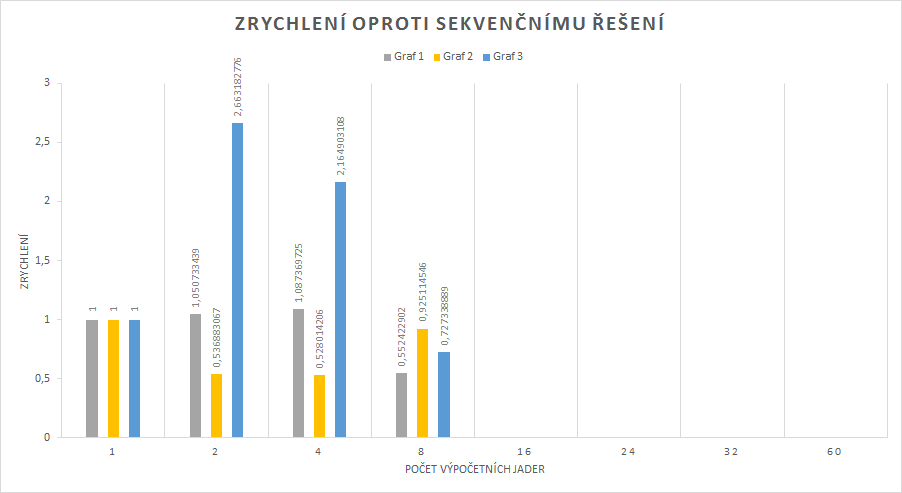
\includegraphics[width=\textwidth]{graph/speedup-chart.png}
\end{figure}

\section{Závěr}

Algoritmus, který jsem naimplementoval v rámci semestrální práce předmětu MI-PDP je korektní a věřím, že po úpravě komunikačního protokolu a experimentování se škálovacími parametry, což jsem popsal výše, se dostanu na lepší časy a lepší zrychlení. 

\appendix

\end{document}